\section{Simulations}

A comprehensive set of subroutines required to compute and evaluate the transfer
functions    outlined    in    this    report    can     be     obtained    from
GitHub\cite{ref:TheComet93}.

The subroutines are located in the folder \textit{matlab/mfunctions}, along with
various utility functions. The folder must be appended to MATLAB's path like so:

\begin{lstlisting}
addpath([pwd,'/mfunctions']);
\end{lstlisting}

This section provides a short overview  of  what  each  subroutine does and how.


\subsubsection*{Pre-processing}

Typically, the  input  data is never perfect. It might contain noise or it might
not have equispaced time values. The function \textit{preprocess\_curve} returns
equispaced time values and smooths the signal.

\begin{lstlisting}
% Smooth input data and generate equispaced
% time vector
[x, y] = preprocess_curve(xr, yr);
\end{lstlisting}

This is achieved  by  using a combination of MATLAB's \textit{smooth()} function
and a custom sliding average  function  to  smooth the beginning and ends of the
signal.


\subsubsection*{Characterising the curve}

With the data prepared (preprocessed), it is now possible to calculate $T_u/T_g$
or $t_{10}$, $t_{50}$, $t_{90}$, depending on  what  you  wish  to  do next. The
function \textit{characterise\_curve()}  can handle both cases for you, like so:

\begin{lstlisting}
% Characterises the curve, either using
% Hudzovic's method or Sani's method.
[Tu, Tg] = characterise_curve(x, y);
[t10, t50, t90] = characterise_curve(x, y);
\end{lstlisting}

Determining $T_u$, $T_g$ is achieved by calculating  the  derivative of the data
to  find  the  point  of  inflection.  The maximum and minimum of the signal  is
determined  by  taking  the  value  of  the  first  and  last  element  in  $y$.

Determining   $t_{10}$,  $t_{50}$,  $t_{90}$  is  achieved  by  using   MATLAB's
\textit{spline()}  function for higher accuracy and  intersecting  the  data  at
10\%, 50\% and 90\% amplitude.  In  the  case of noisy input data, if the spline
fails, the fallback method is to simply find the nearest point. The minimum  and
maximum of the  input  signal  is  again  determined by using the first and last
element in $y$.

Because L. Sani's approach heavily relies  on  accurately  determining the start
and  end  values  of  the input step response function, and it  was  found  that
noisier input  signals  would  significantly  throw  off  correctly  determining
$t_{10}$,  $t_{50}$,  $t_{90}$, it is possible to override the  default  min/max
values by passing in a third argument:

\begin{lstlisting}
% Override Sani's min/max.
ymax = 37;  % Step function stops at 37
ymin = 15;  % Step function starts at 15
[t10, t50, t90] = characterise_curve(x, y, [ymin, ymax]);
\end{lstlisting}

The third argument is only valid for L. Sani's method.

In the case  of  noisy  signals, it is usually better to determine the beginning
and end values of the step response function manually.


\subsubsection*{Calculating T, r and n}

With  $T_u$,  $T_g$  or  $t_{10}$,  $t_{50}$,  $t_{90}$  determined,  the  three
constants $T$, $r$ and $n$ can be calculated using  either  P.  Hudzovic's or L.
Sani's  transfer function (equations \ref{eq:hudzovic}  or  \ref{eq:sani}).  For
this, the two functions  \textit{sani\_lookup()} and \textit{hudzovic\_lookup()}
may be used.

Both  of these functions accept either $T_u/T_g$ or $t_{10}$, $t_{50}$, $t_{90}$
as parameters. Depending  on  which  one  you  choose  to use, the function will
perform a different lookup:

\begin{lstlisting}
% Hudzovic method, Sani method, and their permutations
[T, r, n] = hudzovic_lookup(Tu, Tg);
[T, r, n] = hudzovic_lookup(t10, t50, t90);
[T, r, n] = sani_lookup(t10, t50, t90);
[T, r, n] = sani_lookup(Tu, Tg);
\end{lstlisting}

Note how it's  also  possible  to  use the $t_{10}$, $t_{50}$, $t_{90}$ approach
with  Hudzovic's method,  and  similarly,  use  $T_u/T_g$  with  Sani's  method.

When  calling  these  functions  for  the  first time, they will spend some time
generating  the  lookup  curves  discussed in the theory section. This can  take
about a minute. They are saved to  disk  and  loaded  again if available, so all
subsequent calls will be fast.

The  \textit{sani\_lookup()}  function  will  use  the   interpolation  formulae
(equation  \ref{eq:sani_interpolation})   when   passing   $t_{10}$,   $t_{50}$,
$t_{90}$.   All  other  combinations   will   have   to   use   lookup   curves.


\subsubsection*{Calculating the Transfer Function}

Once    $T$,    $r$    and    $n$    are    obtained,    the    two    functions
\textit{hudzovic\_transfer\_function()}  and \textit{sani\_transfer\_function()}
will help  convert  those  three  constants into a continuous transfer function:

\begin{lstlisting}
% Calculating the transfer functions
G_hudzovic = hudzovic_transfer_function(T, r, n);
G_sani = sani_transfer_function(T, r, n);
\end{lstlisting}

Of  course,  if  the  parameters  $T$,  $r$   and   $n$  were  determined  using
\textit{sani\_lookup()} then  the  function  \textit{sani\_transfer\_function()}
must be used. The same is true for Hudzovic.

Once the transfer function is obtained,  one can view the step response by using
\textit{step()}:

\begin{lstlisting}
% Plot step response
[g, t] = step(G_hudzovic);
plot(t, g);
\end{lstlisting}


\subsubsection*{Fitting}

So  far,  the  typical  work-flow  for  calculating  the transfer function looks
somewhat like the following code:

\begin{lstlisting}
% Hudzovic, Tu/Tg
[Tu, Tg] = characterise_curve(x, y);
[T, r, order] = hudzovic_lookup(Tu, Tg);
G = hudzovic_transfer_function(T, r, order);
\end{lstlisting}

To  further  refine  the result, it is possible to perform a least squares curve
fit  on  a  result  obtained  by  either  method  using   the  \textbf{original}
(non-smoothed)   data.    This    can    be    achieved   with   the   functions
\textit{hudzovic\_fit()} and \textit{sani\_fit()}.

\begin{lstlisting}
% Hudzovic, Tu/Tg, with fitting
[Tu, Tg] = characterise_curve(x, y);
[T, r, n] = hudzovic_lookup(Tu, Tg);
[T, r] = hudzovic_fit(T, r, n, xr, yr);
G = hudzovic_transfer_function(T, r, order);
\end{lstlisting}

Here,  \textit{xr},  \textit{yr}  contain  the  ``raw''  data,  and  \textit{x},
\textit{y} contain the pre-processed (smoothed) data.

Similarly, it is  possible  to  further  refine  a  result obtained by L. Sani's
method using the function \textit{sani\_fit()}:

\begin{lstlisting}
% Hudzovic, Tu/Tg, with fitting
[t10, t50, t90] = characterise_curve(x, y);
[T, r, n] = sani_lookup(t10, t50, t90);
[T, r] = sani_fit(T, r, n, xr, yr);
G = sani_transfer_function(T, r, order);
\end{lstlisting}

The fit is currently not  able  to determine the required order by itself, so it
is necessary to first call \textit{characterise\_curve()} on  the  smoothed data
to retrieve the order. A nice  side  effect  of  doing this is it also gives you
good starting values for $T$ and $r$. This  avoids  the  possibility  of falling
into a local minimum while fitting the data.

\subsection{Reading curves from images}

I have found that more often than not we are required to measure $T_u$ and $T_g$
by  hand from visual plots, without access to the underlying data.  To  overcome
the need to  print  out  the plots onto paper and -- inaccurately -- measure the
data by hand, an algorithm for extracting this data from an image was developed.

\begin{figure}
    \centering
    \begin{subfigure}{.3\textwidth}
        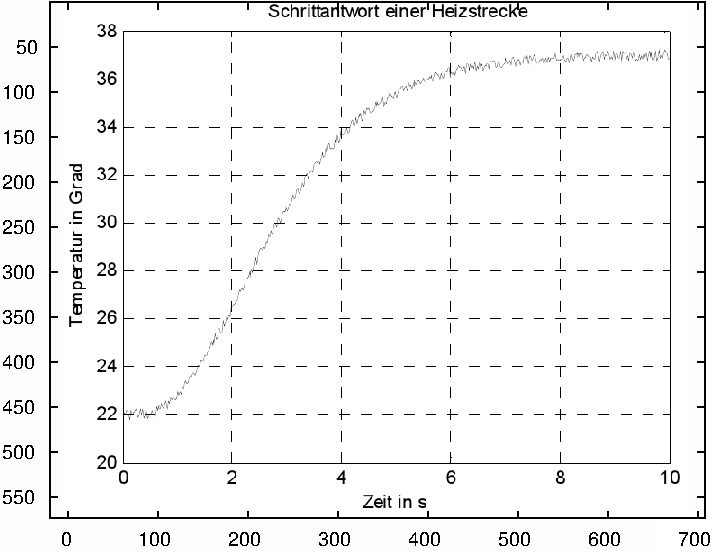
\includegraphics[width=.95\linewidth]{images/plant}
        \caption{Typical image of a plant}
        \label{fig:image:plant}
    \end{subfigure}
    \begin{subfigure}{.3\textwidth}
        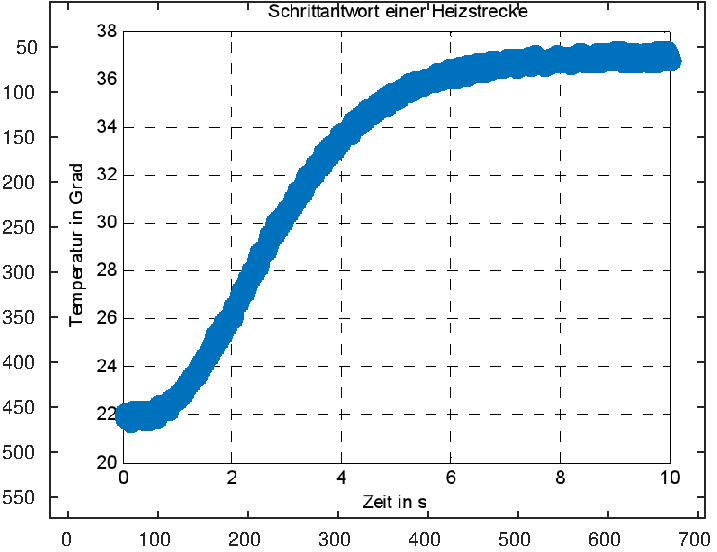
\includegraphics[width=.95\linewidth]{images/scatter_raw}
        \caption{XY scatter of detected data}
        \label{fig:image:scatter_raw}
    \end{subfigure}
    \begin{subfigure}{.3\textwidth}
        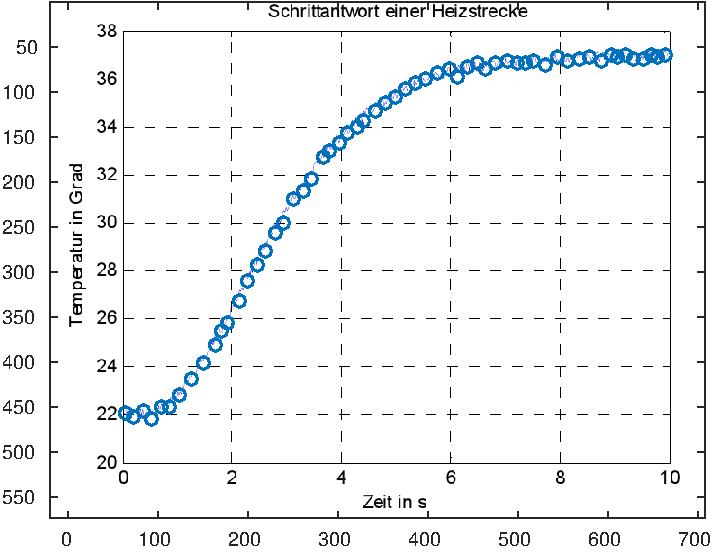
\includegraphics[width=.95\linewidth]{images/scatter_decimated_50}
        \caption{Decimated by 50}
        \label{fig:image:scatter_dec}
    \end{subfigure}
    \caption{Process of importing curve data from an image}
\end{figure}

The algorithm is quite simple: The image data is imported into HSV colour space.
In  the majority of cases, the grid and background will be white, black or  some
grey-scale. The data on the other hand will have a specific colour, which allows
us to first detect  what  the  colour is and then filter the image by hue to get
all data points that have a similar colour.

If the plot happens to be black and white with no colour, then it is possible to
filter  the  data  using  the   ``value''   component   from   the   HSV   data.

The resulting data is usually noisy, but statistically evenly distributed, which
makes  decimation  very easy: Just select every nth data point.  The  data  from
\ref{fig:image:scatter_raw} was decimated by a factor of 50, resulting in figure
\ref{fig:image:scatter_dec}.



